\documentclass[12pt,compress,aspectratio=169]{beamer}

\mode<presentation>
{
  \usetheme{Singapore}
  \setbeamersize{text margin left=.5cm,text margin right=.5cm}
%  \setbeamertemplate{navigation symbols}{} % suppress nav bar
%  \setbeamercovered{transparent}
}
\usefonttheme{professionalfonts}
\usepackage{amsmath,bm}
\usepackage{siunitx}
%\usepackage{graphicx}
\usepackage{tikz}
\usepackage{mathpazo}
\usepackage[scaled]{helvet}
%\usepackage{xcolor,colortbl}
%\usepackage{hyperref}

\sisetup{number-math-rm=\mathnormal}

\title{2.\ Calculus in Physics--Integration}
\subtitle{AP Physics}
\author[TML]{Dr.\ Timothy Leung}
\institute{Olympiads School}
\date{Fall 2017}

\newcommand{\pic}[2]{\includegraphics[width=#1\textwidth]{#2}}
\newcommand{\mb}[1]{\ensuremath\mathbf{#1}}

\begin{document}

\begin{frame}
  \maketitle
\end{frame}

\begin{frame}
  \frametitle{Files for You to Download}
  \begin{itemize}
  \item\texttt{00-outline.pdf}--The course outline
  \item\texttt{01-Calculus-print.pdf}--The slides that I used last week
  \item\texttt{01-integration.pdf}--The slides that I am using right now
  \item\texttt{01-Homework.pdf}--Last/this week's homework assignment
  \end{itemize}
  Please download/print the PDF file for the class slides before each class.
\end{frame}

\section{Differentiation}

\begin{frame}
  \frametitle{On Differential Calculus}
  \framesubtitle{A quick review}
  \begin{itemize}
  \item Finding out how quickly a physical quantity is changing (``rate of
    change'' of that quantity)
  \item Math: slopes of functions
  \item Terminology:
    \begin{itemize}
    \item A \textbf{\emph{derivative}}: The slope of a function (noun)
    \item To \textbf{\emph{differentiate}}: Finding the derivative with respect
      to a variable (verb)
    \end{itemize}
  \item Last class: went through the rules and some examples of derivatives
  \end{itemize}
\end{frame}


\begin{frame}
  \frametitle{Examples of Derivatives in Physics}
  \begin{itemize}
  \item Instantaneous velocity $\mb{v}(t)$ is the derivative of position
    $\mb{s}(t)$
    {\Large
      \begin{displaymath}
        \mb{v}(t)=\frac{d\mb{s}}{dt}
      \end{displaymath}
    }
  \item Instantaneous acceleration $\mb{a}(t)$ is the derivative of velocity
    $\mb{v}(t)$. It's also the ``second derivative'' (derivative of a
    derivative) of position $\mb{s}$ with respect to time
    
    \vspace{-.2in}{\Large
      \begin{displaymath}
        \mb{a}(t)=\frac{d\mb{v}}{dt}=\frac{d^2\mb{s}}{dt^2}
      \end{displaymath}
    }
  \item Instantaneous force $\mb{F}(t)$ is the derivative of momentum
    $\mb{p}$ (Newton's second law of motion)

    \vspace{-.3in}{\Large
      \begin{displaymath}
        \mb{F}(t)=\frac{d\mb{p}}{dt}
      \end{displaymath}
    }
  \end{itemize}
\end{frame}

\begin{frame}
  \frametitle{They're All Vectors}
  \framesubtitle{Resolve them into components}
  \begin{itemize}
  \item Notice that position $\mb{s}$, velocity $\mb{v}$, acceleration $\mb{a}$,
    momentum $\mb{p}$, force $\mb{F}$ are all vector quantities with $x$, $y$
    and $z$ components
  \item In this case, we take the derivative separately in each direction.

    \vspace{-.2in}{\Large
      \begin{displaymath}
        \mb{v}(t)=\frac{d\mb{s}}{dt}
        =\frac{d}{dt}\left[
          s_x(t)\bm{\hat{\imath}}+
          s_y(t)\bm{\hat{\jmath}}+
          s_z(t)\bm{\hat{k}} \right]
      \end{displaymath}
    }
    where $s_x$, $s_y$ and $s_z$ are the $x$-, $y$- and $z$-components of
    $\mb{s}$
  \item In AP or 1st-year physics, $s_x$, $s_y$ and $s_z$ are functions of time
    only, but in practical problems in physics and engineering, they are often
    functions of $x$, $y$ and $z$ coordinates as well. (This is
    \emph{multi-variable calculus}. It's a lot of fun!)
  \end{itemize}
\end{frame}

\begin{frame}
  \frametitle{Other Derivatives}
  \framesubtitle{\ldots Not Always With Respect to Time}
  \begin{itemize}
  \item\textbf{Electric force} is the derivative of electrical potential
    energy with respect to radial distance:

    \vspace{-.3in}{\Large
      \begin{displaymath}
        F_q=-\frac{dU_q}{dr}=-\frac{d}{dr}\left[\frac{kq_1q_2}{r}\right]
      \end{displaymath}
    }

    \vspace{-.1in}Gravitational force and gravitational potential energy are
    related in the same way
  \item\textbf{Electric Field} is the derivative of electric potential
    difference $V$ with respect to the radial distance

    \vspace{-.2in}{\Large
      \begin{displaymath}
        E=-\frac{dV}{dr}
      \end{displaymath}
    }
        
  \end{itemize}
\end{frame}

\begin{frame}
  \frametitle{What the Notation Tells Us}
  \begin{itemize}
  \item When we say we that \textbf{velocity is the time rate of change of
    position}
    {\Large
      \begin{displaymath}
        \mb{v}=\frac{d\mb{s}}{dt}
      \end{displaymath}
    }
  \item We are really asking \textbf{what is the (small) change in position
    $d\mb{s}$ over an infinitesimal (infinitely small) change in time $dt$?}
  \end{itemize}
\end{frame}

\section{Integration}

\begin{frame}
  \frametitle{}
  \begin{center}
    {\LARGE\textbf{NOW ON TO INTEGRATION}}
  \end{center}
\end{frame}

\begin{frame}
  \frametitle{Integral Calculus}
  \begin{itemize}
  \item The opposite of differentiation
  \item We use it to compute the area under a curve, or
  \item Summation of many very small terms
  \item Examples: area under the $\mb{v}$-$t$ graph (to calculate
    displacement), area under the $\mb{F}$-$t$ graph (to calculate impulse),
    area under the $F$-$d$ graph (to calculate work)
  \end{itemize}
\end{frame}


\begin{frame}
  \frametitle{Integration: Area Under the Curve}
  \framesubtitle{Let's start with an example}
  \begin{itemize}
  \item A car moves with speed $v(t)=2+5t$. What is its displacement at $t=5$?
  \item We know that displacement is the area under a $v$-$t$ graph. How do we
    find the area? (Pretend that we don't know the area of a trapezoid!)
  \item Divide the interval from $t=0$ to $5$ into $n$ equal small time
    intervals $\Delta t$
%    \begin{displaymath}
%      \Delta t_1,\;\Delta t_2,\;\Delta t_3,\;\Delta t_4,\ldots,\;\Delta t_n
%    \end{displaymath}
  \item The displacement in each of these $\Delta t_i$ is approximately
    
    \vspace{-.2in}{\large
      \begin{displaymath}
        \Delta s_i = v_i\Delta t
      \end{displaymath}
    }
    
    \vspace{-.3in}where $v_i=v(t_i)$
  \item And the total displacement is:

    \vspace{-0.2in}{\large
      \begin{displaymath}
        \Delta s = \sum_{i=1}^{n}\Delta s_i=\sum_{i=1}^{n} v_i\Delta t
      \end{displaymath}
    }
  \end{itemize}
\end{frame}

\begin{frame}
  \frametitle{Integration: Area Under a Curve}
  \begin{itemize}
  \item Shown graphically:

    \vspace{-0.3in}\begin{center}
      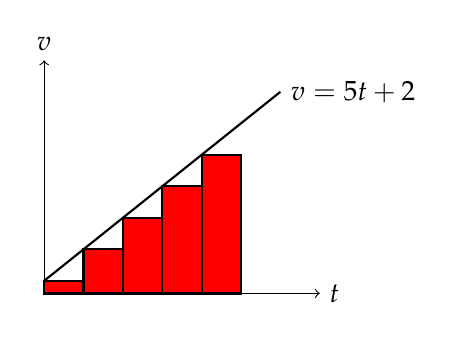
\begin{tikzpicture}[yscale=0.08,xscale=0.5]
        \draw[->](0,0)--(7,0) node[pos=1,right]{$t$};
        \draw[->](0,0)--(0,37) node[pos=1,above]{$v$};
        \foreach \x in {0,1,...,4}{ 
          \pgfmathsetmacro{\y}{5*\x+2};
          \pgfmathsetmacro{\xx}{\x+1};
          \draw[thick,fill=red] (\x,0) rectangle (\xx,\y);
        }
        \draw[thick](0,2)--(6,32) node[pos=1,right]{$v=5t+2$};
      \end{tikzpicture}
    \end{center}
  \item This is not very inspiring, but we can do better if we increase $n$:
    \begin{center}
      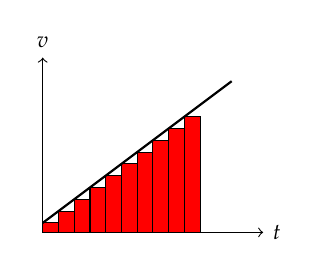
\begin{tikzpicture}[yscale=0.06,xscale=0.4]
        \draw[->](0,0)--(7,0) node[pos=1,right]{\footnotesize $t$};
        \draw[->](0,0)--(0,37) node[pos=1,above]{\footnotesize $v$};
        \foreach \x in {0,0.5,...,4.5}{ 
          \pgfmathsetmacro{\y}{5*\x+2};
          \pgfmathsetmacro{\xx}{\x+0.5};
          \draw[fill=red] (\x,0) rectangle (\xx,\y);
        }
        \draw[thick](0,2)--(6,32);
      \end{tikzpicture}
      \hspace{0.4in}
      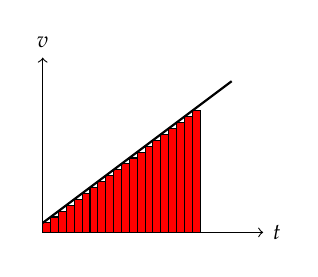
\begin{tikzpicture}[yscale=0.06,xscale=0.4]
        \draw[->](0,0)--(7,0) node[pos=1,right]{\footnotesize $t$};
        \draw[->](0,0)--(0,37) node[pos=1,above]{\footnotesize $v$};
        \foreach \x in {0,0.25,...,4.75}{ 
          \pgfmathsetmacro{\y}{5*\x+2};
          \pgfmathsetmacro{\xx}{\x+0.25};
          \draw[fill=red] (\x,0) rectangle (\xx,\y);
        }
        \draw[thick](0,2)--(6,32);
      \end{tikzpicture}
    \end{center}


  \end{itemize}
\end{frame}

\begin{frame}
  \frametitle{Integration: Area Under a Curve}
  \begin{itemize}
  \item If we increase $n$ to $\infty$, we will have the \emph{actual}
    displacement:

    \vspace{-.2in}{\Large
      \begin{displaymath}
        \Delta s=\lim_{n\rightarrow\infty}\sum_{i=1}^{n}v_i\Delta t
      \end{displaymath}
    }
  \item In fact, this limit is called the integral:
    
    \vspace{-.2in}{\Large
      \begin{displaymath}
        \Delta s=\int_{t_1}^{t_2}v(t) dt
      \end{displaymath}
    }
  \item As $n\rightarrow\infty$, the time interval $\Delta t$ becomes
    infinitesimally small, i.e.\  ``$dt$''
  \end{itemize}
\end{frame}

\begin{frame}
  \frametitle{Integration: Area Under a Curve}
  \begin{itemize}
  \item In our example, we have this particular integral:
    
    \vspace{-.1in}{\large
      \begin{displaymath}
        \Delta s=\int_{t_1}^{t_2}v(t) dt=\int_{0}^{5}(5t+2)\;dt
      \end{displaymath}
    }
  \item How do we compute it?
  \end{itemize}
\end{frame}

\begin{frame}
  \frametitle{The Antiderivative}
  \begin{itemize}
  \item If: $v(t)$ is the derivative of $s(t)$,
  \item Then: $s(t)$ is the ``antiderivative'' of $v(t)$
  \item In general, if $F(x)$ is the antiderivative of $f(x)$, they are related
    this way:
    
    \vspace{-.15in}{\large
      \begin{displaymath}
        \frac{d}{dx}F(x)=f(x)\quad\longrightarrow\quad F(x)=\int f(x)dx
      \end{displaymath}
    }
    %(The mathematical proof is actually the fundamental theorem of calculus.)

  \item If we want to integrate $f(x)$, we are actually asking
    ``what function $F(x)$ has a derivative equal to $f(x)$''?
  \item A simple example with $f(x)=t$ and $F(x)=\frac{1}{2}t^2$:

    \vspace{-0.1in}{\large
      \begin{displaymath}
        \frac{d}{dt}\left(\frac{1}{2}t^2\right)=t
        \quad\longrightarrow\quad
      \int tdt=\frac{1}{2}t^2
      \end{displaymath}
    }
  \end{itemize}
\end{frame}

\begin{frame}
  \frametitle{Commonly Used Integrals in Physics}
  Calculating an integral can be a very daunting task. But these few known
  examples should help in most cases:

  \vspace{-0.3in}{\large
    \begin{align*}
      \int x^ndx&=\frac{1}{n+1}x^{n+1}+C\\
      \int \frac{1}{x}dx &=\ln |x|+C\\
      \int\cos xdx&=\sin x+C\\
      \int\sin xdx&=-\cos x+C
    \end{align*}
  }
  We can ``ignore'' (i.e.\ cancel) the constants $C$ if it is a definite
  integral.
\end{frame}



\begin{frame}
  \frametitle{Definite vs.\ Indefinite Integral}
  \begin{itemize}
  \item An integral can be either ``indefinite'' or ``definite''
  \item An ``indefinite'' integral gives us another function.
  \item For example, given velocity $v(t)$, we can find position $s(t)$
    as a function of time:
    \begin{displaymath}
      s(t)=\int v(t) dt=\cdots + C
    \end{displaymath}
  \item A constant $C$ is added to the anti-derivative of $v(t)$. The exact
    value of $C$ is obtained through applying an ``initial condition'' to the
    problem.
  \item Note: If $s(t)=\mathrm{[something]}+C$ and we take the
    derivative of $s$ to find $v(t)$, the constant term disappears regardless
    of what value it has.
  \end{itemize}
\end{frame}

\begin{frame}
  \frametitle{Definite Integral}
  \begin{itemize}
  \item An integral can also be \textbf{definite},  with lower and upper
    bounds.
  \item For example: given $v(t)$, find displacement between $t=3$ and
    $t=5$:
    \begin{displaymath}
      \Delta s=\int_3^5 v(t)dt
    \end{displaymath}
  \item Once we have computed the integral, we have to evaluate between the
    limits:
    \begin{displaymath}
      \Delta s = s(t)\Big|^5_3=s(5)-s(3)
    \end{displaymath}
  \item In this case we do not have to bother with the constant $C$, since it'll
    cancel out when we evaluate the bounds.
  \end{itemize}
\end{frame}

\begin{frame}
  \frametitle{Back to Our Example}
  \begin{itemize}
  \item The integral in our example is a \emph{definite} integral because it
    has limits $0$ and $5$
  \item We can evaluate it by:
    
    \vspace{-.1in}{\large
      \begin{align*}
        \Delta s&=\int_0^5 (5t+2)\;dt =\int_0^5 5tdt +\int_0^52dt\\
        &= \frac{5}{2}t^2\Big|^5_0+2t\Big|^5_0=\frac{125}{2}+10\\
        &=\boxed{\frac{145}{2}}
      \end{align*}
    }
  \item Each part of the sum can be integrated separately
  \end{itemize}
\end{frame}



\begin{frame}
  \frametitle{Area Under A Curve}
  \framesubtitle{A Math Problem}
  What is the area under the curve
  \begin{displaymath}
    f(x)=2x^2+3x+1\quad\textsf{between}\quad x=1\;\textsf{and}\;x=5
  \end{displaymath}
  Our integration works like this:
  \begin{align*}
    A&=\int_1^5\left(2x^2+3x+1\right)dt\\
    &=\left(\frac{2}{3}x^3+\frac{3}{2}x^2+x\right)\Big|^5_1\\
    &=24+\frac{196}{3}
  \end{align*}
\end{frame}

\section{Kinematics}

\begin{frame}
  \frametitle{Remember Our Kinematic Equations?}
  \begin{itemize}
  \item In Physics 11 and 12, you were introduced to some kinematic equations
    for constant acceleration.
  \item Now that we know something about integration, we can understand these
    equations a little bit better
  \item Start with a constant acceleration $a$. The velocity is the integral:
    
    \vspace{-.2in}{\Large
      \begin{displaymath}
        v(t)=\int adt=at+C
      \end{displaymath}
    }
  \item At $t=0$, $v=v_0$ (``initial value''). Substituting those
    values to find $C=v_0$, and therefore
    
    \vspace{-0.3in}{\Large
      \begin{displaymath}
        \boxed{v(t)=v_0+at}
      \end{displaymath}
    }
  \end{itemize}
\end{frame}

\begin{frame}
  \frametitle{Remember Our Kinematic Equations?}
  \begin{itemize}
  \item Now we integrate $v(t)$ again to get position $s(t)$:
    \vspace{-0.1in}{\Large
      \begin{displaymath}
        s(t)=\int v(t)dt=\int(v_0+at)dt=v_ot + \frac{1}{2}at^2+C
      \end{displaymath}
    }
  \item Again, we take advantage of know our initial position, so $C=s_o$, and
    we have:
    
    \vspace{-0.2in}{\Large
      \begin{displaymath}
        \boxed{s(t)= s_0 + v_ot + \frac{1}{2}at^2}
      \end{displaymath}
    }
  \item You may be more familiar with this expression, where we use
    \emph{displacement} $\Delta s(t) = s(t)-s_0$ instead of position $s$:

    \vspace{-0.25in}{\Large
      \begin{displaymath}
        \Delta s(t)= v_ot + \frac{1}{2}at^2
      \end{displaymath}
    }
  \end{itemize}
\end{frame}

\begin{frame}
  \frametitle{Remember Our Kinematic Equations?}
  \begin{itemize}
  \item In practical situations, acceleration is \emph{not} constant, and we
    generally have to differentiate or integrate to find your answers.
  \end{itemize}
\end{frame}

\begin{frame}
  \frametitle{Other Integrals}
  \begin{itemize}
  \item\textbf{Impulse} (The components of the $\mb{F}$ can be integrated
    separately)
    
    \vspace{-0.2in}{\Large
      \begin{displaymath}
        \mb{J}=\int_{t_1}^{t_2}\mb{F}dt
      \end{displaymath}
    }

  \item\textbf{Work} by non-constant force

    \vspace{-0.25in}{\Large
      \begin{displaymath}
        W=\int_{x_1}^{x_2}\mb{F}(x)\cdot d\mb{s}
      \end{displaymath}
    }
    
    \vspace{-0.1in}This integral is straight forward if $\mb{F}$ is expressed
    as a function of position $\mb{s}$, but if it is written as a function of
    time, i.e.\ $\mb{F}(t)$, then we have to express $\mb{s}$ as a function of
    time as well
  \end{itemize}
\end{frame}


\begin{frame}
  \frametitle{One Last Example}
  \framesubtitle{Work by Non-Constant Force}

  A force of $F(t)=5t\;\si{\N}$ is applied on an object $m=\SI{1}{\kg}$ initially
  at rest, there is no friction force. What would be the displacement and work
  done on this object after \SI{3}{\s}?

  \begin{enumerate}
  \item Apply Newton's second law to find acceleration:
    \begin{displaymath}
      a(t)=\frac{F(t)}{m}=5t
    \end{displaymath}
  \item Then we integrate $a(t)$ with respect with time to get velocity $v(t)$:
    \begin{displaymath}
      v(t)=\int a(t)dt=\frac{5}{2}t^2
    \end{displaymath}
    We already know that $v_0=0$, so we don't have to add $C$ after the
    integral.
  \end{enumerate}
\end{frame}

\begin{frame}
  \frametitle{One Last Example}
  \framesubtitle{Work by Non-Constant Force}

  A force of $F(t)=5t\;\si{\N}$ is applied on an object $m=\SI{1}{\kg}$ initially
  at rest, there is no friction force. What would be the displacement and work
  done on this object after \SI{3}{\s}?

  \begin{enumerate}
    \setcounter{enumi}{2}
  \item We integrate again to get an expression for position $s(t)$:
    \begin{displaymath}
      \Delta s(t)=\int_0^3 v(t)dt=\frac{5}{6}t^3\Big|_0^3
      =\frac{5}{6}\left(3^3-0\right)=\frac{45}{2}\;\si{\metre}
    \end{displaymath}
  \end{enumerate}
\end{frame}

\begin{frame}
  \frametitle{One Last Example}
  \framesubtitle{Work by Non-Constant Force}

  A force of $F(t)=5t\;\si{\N}$ is applied on an object $m=\SI{1}{\kg}$
  initially at rest, there is no friction force. What would be the displacement
  and work done on this object after \SI{3}{\s}?

  \begin{enumerate}
    \setcounter{enumi}{3}
  \item We know from our differential calculus that
    \begin{displaymath}
      v(t)=\frac{ds}{dt}\quad\longrightarrow\quad ds=v(t)dt
    \end{displaymath}
  \item The last step is to integrate force with velocity to find work done.
    (This works because we know $F$ as a function of time.)
    \begin{displaymath}
      W=\int Fds=\int F(t)v(t)dt =\int_0^3\frac{25}{2}t^3dt=\frac{25}{8}t^4\Big|^3_0
      =\frac{2025}{8}=\boxed{253\;\si{J}}
    \end{displaymath}
  \end{enumerate}
\end{frame}

\section{Volume}

\begin{frame}
  \frametitle{Integration to Find Volume}
  \begin{itemize}
  \item Interested in finding the volume when we rotate \emph{any} function
    about the $x$ axis
  \item There are many applications, e.g.\ finding the CG or centroid of shapes
  \end{itemize}
  \begin{columns}
    \column{.33\textwidth}
    \pic{1}{cone.png}
    \column{.64\textwidth}
    \begin{itemize}
    \item Each yellow disk has a volume of $\pi r^2dx$,
      where $r=f(x)$, so the infinitesimal volume $dV$ of each disk is in fact:
      
      \vspace{-0.3in}{\Large
        \begin{displaymath}
          dV=\pi f(x)^{2} dx
        \end{displaymath}
      }    
    \item ``summing'' them together gives us the integral:
      
      \vspace{-0.4in}{\Large
        \begin{displaymath}
          \boxed{V=\int_{x_1}^{x_2} dV=\int_{x_1}^{x_2} \pi f(x)^{2} dx}
        \end{displaymath}
      }
    \end{itemize}
  \end{columns}
\end{frame}



\begin{frame}
  \frametitle{Integration to Find Volume}
  \textbf{Example:} Find the volume of the following shape:
  \begin{itemize}
  \item In this question, $f(x)=3x$, and we are integrating from $x_1=0$ to
    $x_2=1$
  \end{itemize}
  \vspace{.1in}
  \begin{columns}
    \column{.37\textwidth}
    \pic{1}{cone.png}
    \column{.6\textwidth}
    We use the formula from before:
    \begin{align*}
      V&=\int_{x_1}^{x_2} \pi f(x)^{2} dx\\
      &=\int_{0}^{1} \pi 9x^2dx\\
      &=9\pi\int_{0}^{1} x^2dx\\
      &=3\pi x^3\Big|^1_0\\
      &=3\pi
    \end{align*}
  \end{columns}
\end{frame}



\end{document}
